\documentclass[11pt]{article}
\usepackage[utf8]{vietnam}
\usepackage{hyperref}
\usepackage{makecell}
\usepackage{blindtext}
\usepackage{xcolor}
\usepackage{enumitem}
\usepackage{listings}
\hypersetup{
    colorlinks=true, 
    linkcolor=blue,
    filecolor=magenta,      
    urlcolor=red,
    pdftitle={Overleaf Example},
    pdfpagemode=FullScreen,
    }
\usepackage{amsmath,amssymb,amsfonts}
\usepackage{graphicx}

\setlength{\topmargin}{-.5in} \setlength{\textheight}{9.25in}
\setlength{\oddsidemargin}{0in} \setlength{\textwidth}{6.8in}

%%%%%%%%%%%%%%%%%%%%%%%%%%%%%%%%%%%%%%%%%%
\usepackage{pythonhighlight}
%%%%%%%%%%%%%%%%%%%%%%%%%%%
\newcounter{mycounter} % create a new counter, called 'mycounter'
% default def'n of '\themycounter' is '\arabic{mycounter}'
%% command to increment 'mycounter' by 1 and to display its value:
\newcommand\showmycounter{\stepcounter{mycounter}\themycounter}
\usepackage{lipsum}
\newcommand\showlips{\stepcounter{mycounter}\lipsum[\value{mycounter}]}
%%%%%%%%%%%%%%%%%%%%%%%%%%%%%%%%%%%%%%
\usepackage{framed}
\usepackage{hyperref}
\usepackage{fancyhdr}

%%%%%%%%%%%%%%%%%%%%%%%%%%%%%%%%%%%%%%%%%%%%%%%%%%%%%%%%%%%%%
\usepackage{listings}
\usepackage{xcolor}

\definecolor{codegreen}{rgb}{0,0.6,0}
\definecolor{codegray}{rgb}{0.5,0.5,0.5}
\definecolor{codepurple}{rgb}{0.58,0,0.82}
\definecolor{backcolour}{rgb}{0.95,0.95,0.92}

\lstdefinestyle{mystyle}{
    backgroundcolor=\color{backcolour},   
    commentstyle=\color{codegreen},
    keywordstyle=\color{magenta},
    numberstyle=\tiny\color{codegray},
    stringstyle=\color{codepurple},
    basicstyle=\ttfamily\footnotesize,
    breakatwhitespace=false,         
    breaklines=true,                 
    captionpos=b,                    
    keepspaces=true,                 
    numbers=left,                    
    numbersep=5pt,                  
    showspaces=false,                
    showstringspaces=false,
    showtabs=false,                  
    tabsize=2
}

\lstset{style=mystyle}
%%%%%%%%%%%%%%%%%%%%%%%%%%%%%%%%%%%%%%%%%%%%%%%%%%%%%%%%%%%%%
\title{\LARGE AI VIET NAM – COURSE 2022}
\author{\Huge TÊN BÀI BÁO}
\pagestyle{fancy}
\fancyhf{}
\lhead{\bfseries AI VIETNAM}
\rhead{\bfseries  aivietnam.edu.vn}
\begin{document}
\maketitle
%\Large
%\noindent{\bf Ma 12 Long Test 1\hfill 9 February 2017}
%\medskip\hrule

\begin{tabular}{|p{4cm}|p{12cm}|}
 \hline
 \textbf{Ngày công bố:}
  &  11/10/2022 \\
\hline
 \textbf{Tác giả:}
  & Arohan Ajit, Koustav Acharya, Abhishek Samanta  \\
 \hline
 \textbf{Nguồn:} 
  & 2020 International Conference on Emerging Trends in Information Technology and Engineering (ic-ETITE)\\
 \hline
 \textbf{Nguồn dữ liệu (nếu có):} 
  & \href{https://colab.research.google.com/drive/14lyQVNexfDAIqCBDxYhbe0FeslDkefBB?authuser=1}{Link of Data Sources or Name of Data Sources}\\
 \hline
 \textbf{Từ khóa:} 
  & Fault Process and Equipment Analysis, Logistic Regression, Plastic Ball Grid Array Manufacturing Process, Yield Management\\
 \hline
 \textbf{Người tóm tắt:} 
  & TT\\
 \hline
\end{tabular}

\begin{enumerate}
    \item
    \textbf{Mục đích:}
    \begin{itemize}
        \item \blindtext[0]
    \end{itemize}
    
    \item
    \textbf{Đóng góp:}
    \begin{itemize}
        \item \blindtext[0]
    \end{itemize}
    
    \item
    \textbf{Dữ liệu đầu vào:}
    \begin{itemize}
        \item \blindtext[0]
    \end{itemize}
    
    \item
    \textbf{Phương pháp luận:}
    \begin{itemize}
        \item \blindtext[0]
        \item \blindtext[0]
        \begin{figure}[!h]
            \centering
            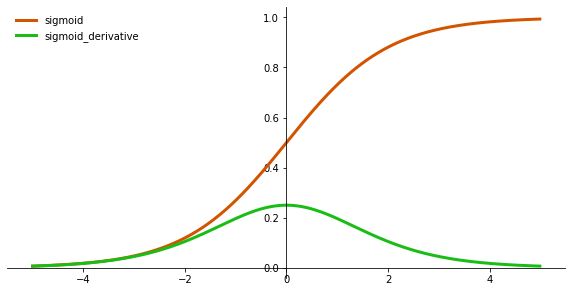
\includegraphics[scale=0.7]{imgs/P1_sigmoid.png}
            \caption{Ví dụ vẽ hình sigmoid và đạo hàm sigmoid}
            \label{fig:P1_sig}
        \end{figure}
    \end{itemize}
    
    \item
    \textbf{Kết quả:}
    \begin{itemize}
        \item \blindtext[0]
        \begin{table}[h]
            \begin{center}
            \caption{Caption}\label{tab:2}
            
            \begin{tabular}{|c|c|c|c|c|}
                \hline
                A & B & C & D & E \\
                \hline
                \hline
                1 & 2 & 3 & 4 & 5 \\
                \hline
        
            \end{tabular}
            \end{center}
        \end{table}
    \end{itemize}
    
    \item
    \textbf{Hạn chế:}
    \begin{itemize}
        \item \blindtext[0]
    \end{itemize}
    
    \item
    \textbf{Các nghiên cứu trong tương lai:}
    \begin{itemize}
        \item \blindtext[0]
    \end{itemize}
    
    \item
    \textbf{Ý tưởng:}
    \begin{itemize}
        \item \blindtext[0]
    \end{itemize}
    
    \item
    \textbf{Ghi chú:}
    \begin{itemize}
        \item \blindtext[0]
    \end{itemize}

         
\end{enumerate}


\end{document} 